\documentclass[tikz, border=4pt]{standalone}
\usepackage{tikz}
\usetikzlibrary{arrows.meta, decorations.pathmorphing, patterns.meta}
\begin{document}
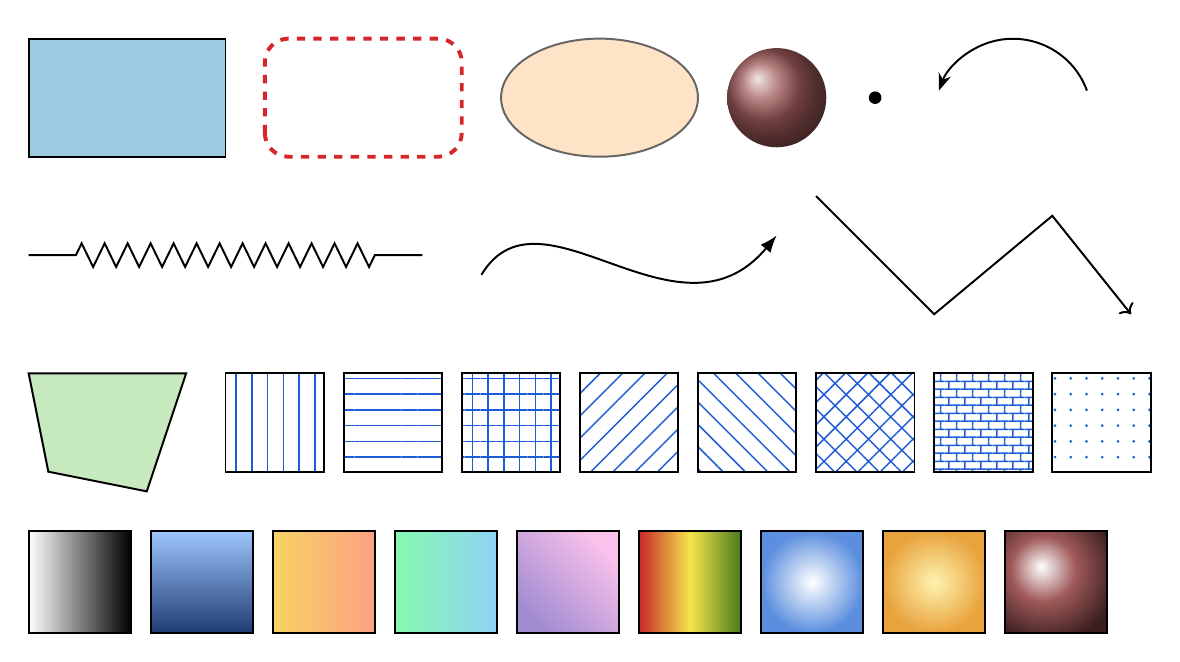
\begin{tikzpicture}[x=1cm, y=1cm]
  \definecolor{tdc1}{HTML}{9ECAE1}
  \definecolor{tdc2}{HTML}{D62728}
  \definecolor{tdc3}{HTML}{FDD0A2}
  \definecolor{tdc4}{HTML}{A05A5A}
  \definecolor{tdc5}{HTML}{C7E9C0}
  \definecolor{tdc6}{HTML}{1E5BD6}
  \pgfdeclarepattern{name=tdbricks0, parameters={}, bottom left={\pgfpoint{0pt}{0pt}}, top right={\pgfpoint{5.69pt}{5.69pt}}, tile size={\pgfpoint{5.69pt}{5.69pt}}, code={\pgfsetlinewidth{0.53pt}\pgfpathmoveto{\pgfpoint{0pt}{1.42pt}}\pgfpathlineto{\pgfpoint{5.69pt}{1.42pt}}\pgfpathmoveto{\pgfpoint{0pt}{4.27pt}}\pgfpathlineto{\pgfpoint{5.69pt}{4.27pt}}\pgfpathmoveto{\pgfpoint{1.42pt}{1.42pt}}\pgfpathlineto{\pgfpoint{1.42pt}{4.27pt}}\pgfpathmoveto{\pgfpoint{4.27pt}{0pt}}\pgfpathlineto{\pgfpoint{4.27pt}{1.42pt}}\pgfpathmoveto{\pgfpoint{4.27pt}{4.27pt}}\pgfpathlineto{\pgfpoint{4.27pt}{5.69pt}}\pgfusepath{stroke}}}
  \pgfdeclarehorizontalshading{tdshade2}{100bp}{rgb(0bp)=(1,1,1); rgb(25bp)=(1,1,1); rgb(75bp)=(0,0,0); rgb(100bp)=(0,0,0)}
  \pgfdeclarehorizontalshading{tdshade3}{100bp}{rgb(0bp)=(0.118,0.235,0.447); rgb(25bp)=(0.118,0.235,0.447); rgb(75bp)=(0.62,0.773,0.996); rgb(100bp)=(0.62,0.773,0.996)}
  \pgfdeclarehorizontalshading{tdshade4}{100bp}{rgb(0bp)=(0.965,0.827,0.396); rgb(25bp)=(0.965,0.827,0.396); rgb(75bp)=(0.992,0.627,0.522); rgb(100bp)=(0.992,0.627,0.522)}
  \pgfdeclarehorizontalshading{tdshade5}{100bp}{rgb(0bp)=(0.518,0.98,0.69); rgb(25bp)=(0.518,0.98,0.69); rgb(75bp)=(0.561,0.827,0.957); rgb(100bp)=(0.561,0.827,0.957)}
  \pgfdeclarehorizontalshading{tdshade6}{100bp}{rgb(0bp)=(0.631,0.549,0.82); rgb(25bp)=(0.631,0.549,0.82); rgb(75bp)=(0.984,0.761,0.922); rgb(100bp)=(0.984,0.761,0.922)}
  \pgfdeclarehorizontalshading{tdshade7}{100bp}{rgb(0bp)=(0.776,0.157,0.157); rgb(25bp)=(0.776,0.157,0.157); rgb(50bp)=(0.961,0.894,0.298); rgb(75bp)=(0.29,0.478,0.118); rgb(100bp)=(0.29,0.478,0.118)}
  \pgfdeclareradialshading{tdshade8}{\pgfpoint{0bp}{0bp}}{rgb(0bp)=(1,1,1); rgb(25bp)=(0.357,0.557,0.871); rgb(100bp)=(0.357,0.557,0.871)}
  \pgfdeclareradialshading{tdshade9}{\pgfpoint{0bp}{0bp}}{rgb(0bp)=(1,0.953,0.69); rgb(25bp)=(0.91,0.639,0.239); rgb(100bp)=(0.91,0.639,0.239)}
  \pgfdeclareradialshading{tdshade10}{\pgfpoint{-7.5bp}{7.5bp}}{rgb(0bp)=(1,1,1); rgb(15.75bp)=(0.627,0.353,0.353); rgb(35bp)=(0.227,0.114,0.114); rgb(100bp)=(0.227,0.114,0.114)}

  \draw[line width=0.71pt, fill=tdc1] (0,-1.5) rectangle (2.5,0);
  \draw[draw=tdc2, line width=1.42pt, dashed, rounded corners=8.54pt] (3,-1.5) rectangle (5.5,0);
  \begin{scope}[transparency group, opacity=0.6]
    \draw[line width=0.71pt, fill=tdc3] (7.25,-0.75) ellipse (1.25 and 0.75);
  \end{scope}
  \shade[ball color=tdc4] (9.5,-0.75) circle (0.63);
  \fill (10.75,-0.75) circle (0.08);
  \draw[line width=0.71pt, -{Stealth}] (13.44,-0.66) arc[start angle=20, end angle=160, radius=1];
  \draw[line width=0.71pt, decorate, decoration={zigzag, segment length=0.292cm, amplitude=0.15cm, pre length=0.6cm, post length=0.6cm}] (0,-2.75) -- (5,-2.75);
  \draw[line width=0.71pt, -{Latex}] (5.75,-3) .. controls (6.5,-1.75) and (8.25,-4) .. (9.5,-2.5);
  \draw[line width=0.71pt, -{To}] (10,-2) -- (11.5,-3.5) -- (13,-2.25) -- (14,-3.5);
  \draw[line width=0.71pt, fill=tdc5] (0,-4.25) -- (2,-4.25) -- (1.5,-5.75) -- (0.25,-5.5) -- cycle;
  \draw[line width=0.71pt, pattern={Lines[angle=90, distance=5.69pt, line width=0.53pt]}, pattern color=tdc6] (2.5,-5.5) rectangle (3.75,-4.25);
  \draw[line width=0.71pt, pattern={Lines[angle=0, distance=5.69pt, line width=0.53pt]}, pattern color=tdc6] (4,-5.5) rectangle (5.25,-4.25);
  \draw[line width=0.71pt, pattern={Hatch[angle=0, distance=5.69pt, line width=0.53pt]}, pattern color=tdc6] (5.5,-5.5) rectangle (6.75,-4.25);
  \draw[line width=0.71pt, pattern={Lines[angle=45, distance=5.69pt, line width=0.53pt]}, pattern color=tdc6] (7,-5.5) rectangle (8.25,-4.25);
  \draw[line width=0.71pt, pattern={Lines[angle=-45, distance=5.69pt, line width=0.53pt]}, pattern color=tdc6] (8.5,-5.5) rectangle (9.75,-4.25);
  \draw[line width=0.71pt, pattern={Hatch[angle=45, distance=5.69pt, line width=0.53pt]}, pattern color=tdc6] (10,-5.5) rectangle (11.25,-4.25);
  \draw[line width=0.71pt, pattern=tdbricks0, pattern color=tdc6] (11.5,-5.5) rectangle (12.75,-4.25);
  \draw[line width=0.71pt, pattern={Dots[distance=5.69pt, radius=0.53pt]}, pattern color=tdc6] (13,-5.5) rectangle (14.25,-4.25);
  \draw[line width=0.71pt, shade, shading=tdshade2] (0,-7.55) rectangle (1.3,-6.25);
  \draw[line width=0.71pt, shade, shading=tdshade3, shading angle=90] (1.55,-7.55) rectangle (2.85,-6.25);
  \draw[line width=0.71pt, shade, shading=tdshade4] (3.1,-7.55) rectangle (4.4,-6.25);
  \draw[line width=0.71pt, shade, shading=tdshade5] (4.65,-7.55) rectangle (5.95,-6.25);
  \draw[line width=0.71pt, shade, shading=tdshade6, shading angle=45] (6.2,-7.55) rectangle (7.5,-6.25);
  \draw[line width=0.71pt, shade, shading=tdshade7] (7.75,-7.55) rectangle (9.05,-6.25);
  \draw[line width=0.71pt, shade, shading=tdshade8] (9.3,-7.55) rectangle (10.6,-6.25);
  \draw[line width=0.71pt, shade, shading=tdshade9] (10.85,-7.55) rectangle (12.15,-6.25);
  \draw[line width=0.71pt, shade, shading=tdshade10] (12.4,-7.55) rectangle (13.7,-6.25);
\end{tikzpicture}
\end{document}
